\documentclass[12pt,a4paper]{scrreprt}
\usepackage[T1]{fontenc}
\usepackage[utf8]{inputenc}
\usepackage[ngerman]{babel}
%damit Tabellen direkt an der Stelle im Latex-Code auftauchen [H]
\usepackage{float}
%Zur Einbindung von Grafiken benötigt
\usepackage{graphicx}
%für Referenzen
\usepackage[backend=bibtex8, subentry]{biblatex}
%Verlinkungen für Inhaltsverzeichnis
\usepackage[colorlinks = true, linkcolor = black, citecolor = black, filecolor = black, urlcolor = black]{hyperref}
%Paket für Schriftarten
\usepackage{listings} 
%SQL-Schriftart
\lstset{language=Java,basicstyle=\footnotesize}

%bindet die source.bib ein
\bibliography{source}

%keine Einrückungen
%\setlength{\parindent}{0pt}

\begin{document}

% Titelblatt der Arbeit
  \begin{titlepage}

	\vspace*{0.5cm}

 \begin{center} \large 
    
    \huge {Universität Leipzig} \\
    \large Fakultät für Mathematik und Informatik \\
    Institut für Informatik \\
    \vspace*{2cm}

    {\huge Erstellen einer Webseite \\
    \vspace*{0.2cm}
    \huge für die Badminton-Domäne}
    \vspace*{1.5cm}

    Christoph Beger und Marcel Jacob \\ 
    \vspace*{0.5cm}
    angefertigt in der Abteilung Automatische Sprachverarbeitung
    \vspace*{1.5cm}

    Leipzig, den \today
    \vspace*{3cm}
    
  \end{center}
\end{titlepage} 
\newpage

%Inhaltsverzeichnis erstellen
\tableofcontents 
\newpage

\chapter{Einleitung}
\section{Gegenstand und Motivation}
\subsection{Gegenstand}
Jede moderne, dynamische Website arbeitet mit einer oder mehreren Datenbanken als Datenbasis. Dadurch ist es leicht möglich die Webseiten flexibler und erweiterbar zu gestalten. Die Anzahl der Webseiten, die in reinem HTML-Code geschrieben sind, ist mittlerweile verschwindend gering geworden, da dies zu statisch ist. 

\subsection{Problematik}
Trotz der Fülle an vorhandenen Datenbanken im Netz, ist nur ein Bruchteil davon offen zugänglich. Dies kann beispielsweise aus Datenschutzgründen geschehen, um die privaten Informationen von Kunden vor fremden Zugriffen zu bewahren, oder aus Profitgründen, wenn ein Unternehmen mit den vorhandenen Daten Geld verdient. 

Die Daten sind also schlecht zugänglich und daher nicht für Analysezwecke geeignet. Außerdem besteht nicht die Möglichkeit Daten aus verschiedenen Quellen für eine Analyse zu vereinigen. 

\subsection{Motivation}
Da man aber beispielsweise über das Web-Interface viele Daten abgreifen kann, ist es möglich die vorhandenen Informationen aufzubereiten und eine eigene Datenbank für diese zu erstellen. Dieses Szenario lässt sich auf eine Vielzahl von Domänen anwenden. In dieser Arbeit liegt der Fokus auf einer speziellen Domäne: Badminton. Wie auch in anderen Sportarten, gibt es eine Weltrangliste für Teams oder einzelne Spieler, die von einer Organisation verwaltet und regelmäßig aktualisiert wird. Für die Rangliste beim Badminton ist die Badminton World Federation (BWF) zuständig, welche über folgenden Link erreicht werden kann: http://bwf.tournamentsoftware.com/home.aspx \cite{BWF2015}

\section{Zielsetzung}
Ziel der Arbeit soll es sein, die entsprechenden HTML-Dokumente für die einzelnen Spieler herunterzuladen, aus diesen die relevanten Daten zu extrahieren und in eine eigenkonzipierte Datenbank zu importieren, um im Anschluss ein Webfrontend für eine angemessene Repräsentation und Zugänglichkeit der Informationen zu erstellen.
\newpage

\chapter{Grundlagen}
\section{Django}
\label{Django}
Django ist ein Framework, mit dessen Hilfe Websiten erstellt werden können. Dafür setzt Django auf die Programmiersprache Python und legt Wert auf Wiederverwendbarkeit der einzelnen Komponenten. Es folgt einem Model-Template-View Muster, welches sich an dem Model-View-Controller Schema orientiert. Mit Hilfe eines objekt-relationalen Mappers (ORM) werden die geschriebenen Models in Datenbankstrukturen überführt und die Anfragen ausgeführt. Zum Testen der erstellten Webseite bringt Django einen Entwicklungs-Webserver mit. Django wird derzeit aktiv entwickelt, die neueste Version ist die 1.7.4 (Stand 18. Februar 2015).

\section{PostgreSQL}
Als Daten haltendes Backend haben wir das objektrelationale Datenbankmanagementsystem (DBMS) PostgreSQL (siehe \cite{PostgreSQL2015}) ausgewählt. Das DBMS ist open-source und unterstützt einen großteil des SQL-Standards. Zudem lässt sich PostgreSQL um eine Vielzahl von eigenentwickelten Komponenten erweitern.\\

\noindent Beispielsweise können folgende Komponenten selbst definiert werden:
\begin{itemize}
\item Datentypen
\item Funktionen
\item Operatoren 
\item u.v.m.
\end{itemize}

\chapter{Vorüberlegungen}
\section{Crawling und Parsing relevanter Webseiten}
Warum, welche Seiten crawlen? -> biography-Seiten
Auf HTML-Struktur der Seiten kurz eingehen.
Lokalisierung relevanter Informationen, evtl. mit Screenshot.

\section{Gestaltung des Frontends}
Search-Seite mit einer Liste aller Player:

paging (Auswahl players per page)
Sortierung nach Spalten
Filter-/Suchfunktion (Für alle Attribute entsprechende Filtermöglichkeiten)
evtl. Möglichkeit für Auswahl der Sichtbaren Attribute
http://django-filter.readthedocs.org/en/latest/usage.html https://django-tables2.readthedocs.org/en/latest/

Details-Seite für ausgewählten Player:

Darstellung aller Informationen zu Player
Einbindung von Bildern
(evtl. Grafik zum Rankingverlauf)
Attribute aus externen Tabellen z.B. club, nationality als Link auf Search-Seite, wo alle Player mit dem jeweiligen Attribut aufgelistet werden
Bearbeitungsfunktion für Felder mit NULL-Werten -> wäre Edit-Seite nötig (nur Informationen hinzufügen)
Query-Seite zur erstellen von Abfragen

Result-Seite für die Darstellung der Ergebnisse:

Grafikgenerierung: Häufigkeiten ( Player.objects.values\_list('FIELD').annotate(count=Count('FIELD')).values\_list('count') )
Ergebnis mit Player-Menge als Redirect auf Search-Seite

\chapter{Umsetzung}
\section{Systemvoraussetzungen}
Django-Installation, Pakete

\section{Aufbau des Backend}
\label{Backend}
Zunächst musste ein Crawler geschrieben werden, der die entsprechenden Webseiten herunterlädt und abspeichert. Diesen Schritt haben wir mit Hilfe von Java umgesetzt. Da es den Anschein hatte, dass die Webseite den Zugriff nach ca. 100 Dokumenten verweigert, wurde der Crawler um eine Funktion erweitert, mit deren Hilfe man einen Webproxy zwischenschalten kann, der dieses Problem löst. Sobald ein Dokument nicht heruntergeladen werden kann, wird der nächste Proxy aus der Liste genommen. Die Proxy-Liste stammt von http://proxylist.hidemyass.com/ \cite{HMA2015}. Insgesamt wurden 7854 Dokumente heruntergeladen.\\

Im nächsten Schritt wurde ein Perl-Skript geschrieben, welches die vorhandenen Informationen extrahiert und in eine PostgreSQL Datenbank importiert. Hierfür wurde vorher ein entsprechendes Schema, welches in der folgenden Abbildung dargestellt ist, erstellt. Das Schema spiegelt die Informationen wider, die extrahiert und für den Import in die Datenbank normalisiert wurden. Hierzu zählen beispielsweise Informationen wie Geburtstag, Geburtsort, Größe und Links-/Rechtshänder.

\begin{figure}[H]
\centering
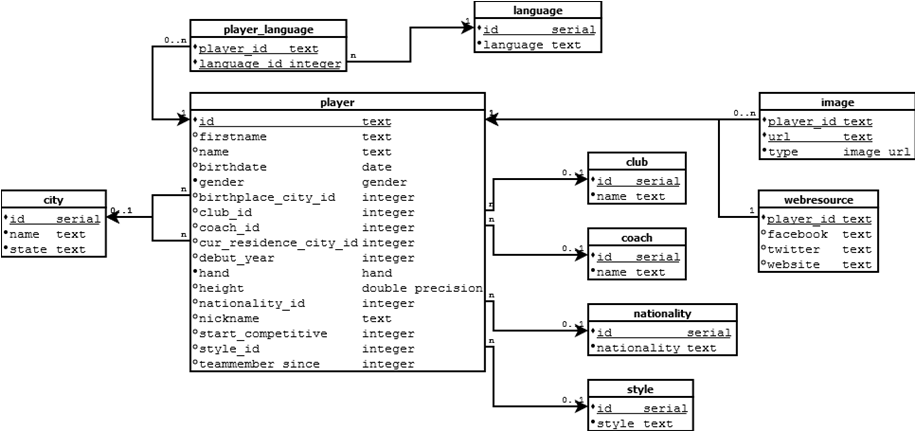
\includegraphics[width=1\textwidth] {ER-Diagramm} 
\caption{ER-Diagramm}
\label{fig:ER-Diagramm}
\end{figure}

\section{Aufbau des Frontend}
\label{Frontend}
Die erstellte Webseite soll gut lesbar, schnell zu laden und intuitiv zu bedienen sein. Dafür wurde auf der Startseite ein kleines Navigationsmenü zur Unterteilung der einzelnen Features eingerichtet. Auf der Startseite erhält man einen kleinen Begrüßungstext, der das Ziel und die Funktionen der Webseite kurz beschreibt. Mit dem Suchformular ist es möglich, nach Spielern zu suchen, die gewisse Bedingungen erfüllen. Klickt man auf die etwas längliche Spieler-Id, werden alle wichtigen Informationen und, wenn vorhanden ein Bild des Spielers, angezeigt. Hier ist es auch möglich bestimmte Informationen für den Spieler zu setzen, wenn diese noch \glqq NULL\grqq{} sind. Sucht man beispielsweise nach dem deutschen Badmintonspieler Marc Zwiebler, ist es nur möglich den Verein einzutragen, da alle anderen Werte bereits gesetzt sind und viele Werte wie Geburtstag, Name und Geschlecht sich im Laufe des Lebens nicht ändern.

Außerdem gibt es eine Reihe von vordefinierten Statistiken, die auf Basis der Datenbank erstellt wurden. Hierzu zählen:
Links- vs. Rechtshänder, Verein, Coach, Disziplin, Geschlecht, gesprochene Sprache / Muttersprache, aktuelle Nationalität und die Körpergröße. Zu guter Letzt gibt es einen Editor, mit dem Nutzer SQL-Anfragen schreiben können, um ihre eigenen Informationsbedürfnisse zu stillen.

\chapter{Erkenntnisse}
\label{Erkenntnisse}
Laut dem NTV-Artikel \cite{Hand2015}, wird der Anteil der Linkshänder in der Bevölkerung auf 10 bis 15\% geschätzt, ihr Anteil läge im Spitzensport in einigen Sportarten aber bei bis zu 55\%. Betrachtet man nun unsere mageren 8,81\% für den Anteil der Linkshänder, bekommt man den Eindruck, dass die Linkshänder im Nachteil wären. Eine kurze manuelle Auswertung der aktuellen Weltrangliste (Stand 18. Februar 2015) für das Herren- und das Dameneinzel für die ersten 25. Plätze, ergibt jedoch einen höheren Anteil der Linkshänder. Bei den Männern sind 6 der 25 Topleute Linkshänder, bei den Frauen sind es immerhin 4. Dies ergibt einen Anteil von 20\%, welcher immerhin etwas über dem Anteil an der Gesamtbevölkerung liegt und den vermeintlichen Nachteil in einen Vorteil wandelt. Dennoch sind die Daten mit Vorsicht zu genießen, da ebenfalls die Top-100 hätten ausgewertet werden können, was in der Folge wiederum zu anderen Zahl führt.

Für die Geschlechterverteilung ergibt sich ein geringes Ungleichgewicht zugunsten der Männer, die 59,8\% einnehmen. Bei der Länderverteilung belegt Indonesien mit 521 Spitzensportlern den ersten Platz, gefolgt von Großbritannien mit 363 Spielern. Deutschland belegt mit 199 Spielern den 9. Rang. Insgesamt lässt sich ein Trend in den asiatischen Ländern und in Europa erkennen, welche einen Großteil aller Spieler einnehmen.\\

Bei den Statistiken zu dem Verein, dem Coach, der gesprochenen Sprache und der Körpergröße lässt sich sagen, dass hier nur sehr wenige Daten vorhanden sind. Daher lässt sich keine allgemeine Aussage für diese Werte treffen.

\section{Fehler und Verbesserungsmöglichkeiten}
Der selbst geschriebene Crawler hält sich nicht an gängige Richtlinien, die ein \glqq richtiger\grqq{} Crawler einhalten würde. Beispielweise müsste man nach einer \glqq robots.txt\grqq{} suchen, damit man weiß welche Dokumente crawlen darf und welche nicht. Außerdem müsste sich ein Crawler im HTTP-Protokoll im Feld \glqq user-agent\grqq{} erkennbar machen, da es sich nicht um einen normalen Nutzer handelt, sondern um ein gefräßiges Datenmonster :D Um den Server nicht zu überlasten, müssten Wartezeiten eingehalten werden, bevor das nächste Dokument gecrawlt werden kann.\\

Im Bereich des Profil-Updates sind einige Verbesserungsmöglichkeiten denkbar. Man könnte beispielsweise ein Update für alle Werte erlauben, die sich im Laufe eines Lebens ändern können, auch wenn diese bereits gesetzt sind. Hierzu zählt auch der Nachname, der sich bei einer Heirat ändern kann. Für die Qualität der Datenbank wäre es wichtig, die geänderten Werte nicht einfach zu übernehmen, sondern als Vorschläge in einer gesonderten Tabelle abzuspeichern und manuell überprüfen zu lassen.\\

Verein, Coach als Text? Größe nur im Bereich 100-220 cm?

\section{Erweiterungsmöglichkeiten}
Es wäre denkbar die Webseite zu \glqq vervollständigen\grqq, da in der Datenbank noch viele Informationen zu den Spielern leer sind. Dafür könnte man weitere Seiten crawlen und parsen, um den die Lücken im Datenbestand zumindest teilweise zu schließen. Außerdem lassen sich weitere Informationen in die Webseite einpflegen. Beispielsweise könnten die Regeln für Badminton ergänzt oder interessante Matches zwischen den Top-Spielern als Video eingebettet werden. Selbstverständlich sind weitere Möglichkeiten für die Visualisierungen mit den vorhandenen Daten denkbar.

\chapter*{Zusammenfassung}
\addcontentsline{toc}{chapter}{Zusammenfassung}
Durch den Einsatz verschiedener Technologien und Werkzeuge ist es gelungen, aus schlecht zugänglichen Daten eine Webseite zu erstellen, die interessante Aspekte der Daten visualisieren kann. Im gesamten Prozess der Entwicklung ging es auch um das Kennenlernen neuer Technologien, vor allem im Bereich Webdesign.

\newpage

\chapter*{Literaturverzeichnis}
\addcontentsline{toc}{chapter}{Literaturverzeichnis}
\printbibliography	
\newpage

\newpage

\end{document}
